\documentclass[12pt]{report}
\usepackage[utf8]{inputenc}


%\pagenumbering{Roman}
%\renewcommand\thepage{\arabic{page}}
\usepackage{ragged2e}
\usepackage{graphicx,float}
\usepackage{wrapfig}
\usepackage{hyperref}
\usepackage[margin=1in]{geometry}
\usepackage{subcaption}
% \usepackage{subfigure}
\usepackage{xcolor}
\usepackage{tikz}
\usepackage{amssymb}
%\usepackage{makecell}
\usepackage{multirow}
%\usepackage{boldline} 
\usepackage{array}
\usepackage{booktabs}
\usepackage{siunitx}
\usepackage{cite}
\usepackage{setspace}
\usepackage[nottoc,notlot]{tocbibind}
\usepackage{blindtext}
\usepackage{cancel} % for cancelto method

\setlength{\parskip}{1em}
\usepackage[most]{tcolorbox}

\graphicspath{ {../images/} }

% define matplotlib colors
\definecolor{darkgreen}{rgb}{0.0, 0.5, 0.0}



\usepackage{titling}
\newcommand{\proposalTitle}{Efficient Deep Learning for Massive MIMO Channel State Estimation}
\newcommand{\authorName}{Mason del Rosario}
\newcommand{\authorDepartment}{Electrical and Computer Engineering}
\newcommand{\authorUniversity}{University of California, Davis}
\newcommand{\authorAddress}{Davis, CA 95616}
\newcommand{\authorEmail}{mdelrosa@ucdavis.edu}

\title{}

\author{
	\authorName\\
	%  <Department> of Electrical and Computer Engineering\\
	\authorDepartment\\
	\authorAddress \\ % in US, this will be <City>, <State> <ZIP> for University
	\authorEmail \\
}

\date{\today}

\doublespacing

\begin{document}
	
% 00_title.tex

\begin{titlepage}
	\null\vfill
	
	\begin{center}
		
		{\Huge \proposalTitle}
		\vskip 2cm
		
		{\Large \authorName}
		\vskip 1cm
		
		{\large \authorUniversity\\
				\authorAddress \\
				\texttt{\authorEmail} \\}
	\end{center}
	
	\vfill
	\vfill
	
	\centering
	\begin{tabular}{r}
		\today \\
	\end{tabular}
\end{titlepage}



\newpage
\tableofcontents

\newpage

\chapter{Introduction}
% 01_introduction.tex

Here is an example of a citation \cite{ref:oetiker1995not}. Citations are included in the \texttt{cited\_works.bib} file.

\subsection{MIMO Channel Overview}
\label{sect:mimo_model}

In this work, we consider a MIMO channel with a multiple antennas ($n_B \gg 1$) at the transmitter (gNodeB or gNB) servicing a single (or multiple) user equipment(s) (UE) with a single antenna. The network utilizes orthogonal frequency division multiplexing (OFDM) with $N_f$ subcarriers, the $m$-th downlink and uplink channels at the receiver are given as
\begin{align*}
	y_{d,m} &= \mathbf h_{d,m}^H\mathbf w_{t,m}x_{d,m} + n_{d,m}, \\
	y_{u,m} &= \mathbf w_{r,m}^H\mathbf h_{u,m}x_{u,m} + \mathbf w_{r,m}^H\mathbf n_{u,m}.
\end{align*}
The resulting downlink and uplink channel state information (CSI) matrices are given as
\begin{align*} 
	\bar{\mathbf H}_d &= \begin{bmatrix} \mathbf h_{d,1} & \dots & \mathbf h_{d,N_f}\end{bmatrix}^H \in \mathbb C^{N_f \times N_b}, \\
	\bar{\mathbf H}_u &= \begin{bmatrix} \mathbf h_{u,1} & \dots & \mathbf h_{u,N_f}\end{bmatrix}^H \in \mathbb C^{N_f \times N_b}.
\end{align*}
\begin{table}[]
\centering
\caption{MIMO system parameters and variables considered in this work.}
\label{tab:cost-params}
\begin{tabular}{c|c|l}
\toprule
\textbf{Symbol}   & \textbf{Dimension}          & \textbf{Description} \\ \midrule
$y_{d,m}$ 		  & $\mathbb{C}^{1}$ 			& Received downlink symbol on $m$-th subcarrier  \\ \hline
$\mathbf h_{d,m}$ & $\mathbb{C}^{N_b \times 1}$ & Downlink impulse response on $m$-th subcarrier  \\ \hline
$\mathbf w_{t,m}$ & $\mathbb{C}^{N_b \times 1}$ & Transmitter precoding vector for $m$-th subcarrier  \\ \hline
$x_{d,m}$ 		  & $\mathbb{C}^{1}$ 			& Trasmitted symbol on $m$-th subcarrier  \\ \hline
$n_{d,m}$ 		  & $\mathbb{C}^{1}$ 			& Downlink noise on $m$-th subcarrier  \\ \hline
$y_{u,m}$ 		  & $\mathbb{C}^{1}$ 			& Received uplink symbol on $m$-th subcarrier  \\ \hline
$\mathbf h_{u,m}$ & $\mathbb{C}^{N_b \times 1}$ & Uplink impulse response on $m$-th subcarrier  \\ \hline
$\mathbf w_{r,m}$ & $\mathbb{C}^{N_b \times 1}$ & Received precoding vector for $m$-th subcarrier  \\ \hline
$x_{u,m}$ 		  & $\mathbb{C}^{1}$ 			& Received symbol on $m$-th subcarrier  \\ \hline
$\mathbf n_{u,m}$ & $\mathbb{C}^{1}$ 			& Uplink noise on $m$-th subcarrier  \\ \hline
\end{tabular}
\end{table}
To achieve near-capacity transmission rates, the transmitter needs access to an appropriate estimate of $\bar{\mathbf H}_d$ \cite{ref:goldsmith2003capacity}. In time division duplex (TDD), downlink CSI estimation can be performed by using pilots in uplink frames due to channel reciprocity. In contrast, frequency domain duplex (FDD) does not admit channel reciprocity due to frequency-selective channels, and CSI estimates must be acquired using feedback.

Given their dimensionality, feeding back entire CSI matrices is impractical. Instead, we seek a compressed representation of a sparse transformation. We consider the angular-delay representation of CSI matrices. Denote the unitary DFT (inverse DFT) matrix $\mathbf F \in \mathbb C^{n_f \times n_f}$ ($\mathbf F^H \in \mathbb C^{n_f \times n_f}$), and denote the spatial-frequency CSI matrix as $\bar{\mathbf H}$. The angular-delay domain representation $\mathbf H$ is given as
\begin{align*}
	\mathbf H &= \mathbf F^H \bar{\mathbf H} \mathbf F
\end{align*}

\subsection{Channel Model}
\label{sect:channel_model}

For all CSI tests, we mainly rely on the COST2100 MIMO channel model \cite{ref:liu2012cost2100}. We use two datasets with a single base station (gNB) and a single user equipment (UE) in the following scenarios:
\begin{enumerate}
	\item \textbf{Indoor} channels using a 5.3GHz downlink at
	0.001 m/s UE velocity, served by a
	gNB at center of a $20$m$\times 20$m coverage area.
	\item \textbf{Outdoor} channels using a 300MHz downlink at 0.9 m/s UE velocity served by a gNB at center 
	of a $400$m$\times 400$m coverage area.
\end{enumerate}
In both scenarios, we use the parameters listed in Table~\ref{tab:cost-params}.
\begin{table}[]
\centering
\caption{Parameters used for COST2100 simulations for both Indoor and Outdoor datasets.}
\label{tab:cost-params}
\begin{tabular}{c|c|l}
\toprule
\textbf{Symbol} & \textbf{Value} & \textbf{Description} \\ \midrule
$N_b$ 			& 32			 & Number of antennas at gNB  \\ \hline
$N_f$ 			& 1024			 & Number of subcarriers for OFDM link  \\ \hline
$R_d$ 			& 32			 & Number of delay elements kept after truncation  \\ \hline
$N$ 			& $10^6$		 & Total number of samples per dataset  \\ \hline
$T$ 			& 10		 	 & Number of timeslots  \\ \hline
$\delta$		& 40ms, 80ms	 & Feedback delay interval between consecutive CSI timeslots  \\ \bottomrule
\end{tabular}
\end{table}


\chapter{Data Pre-processing and Normalization}
\label{chap:sph_norm}
% 03_sph_norm.tex

In this chapter, we will discuss the data pre-processing techniques and the applications of domain knowledge that have enabled successful application of deep learning to MIMO CSI estimation (Section~\ref{sec:data-preprocessing}), including our proposed pre-processing technique, spherical normalization (Section~\ref{sect:sph_norm}). 

% For data with multiple input features of different scales. In ML curricula, this is often illustrated using the iris dataset \cite{ref:anderson1936species,ref:fisher1936use}), which contains .

\section{Data Pre-processing for CSI Data} \label{sec:data-preprocessing}

The success of machine learning tasks relies on proper \emph{data pre-processing}, a sequence of transformations used on the input data before fitting a model. In any machine learning task, data pre-processing is necessary to ensure that the scales of input features are similar. In deep learning, three important pre-processing techniques are domain transformations, truncation, or normalization, and here we will explore the choices in pre-processing that different authors have made based on domain knowledge of MIMO CSI data.

\subsection{Sparse Basis for CSI}

\begin{figure}[htb]
	\centering
	\includegraphics[width=.8\textwidth]{batch17_sample0_freqvsdel_truncatevsfull.pdf}
	\medskip
	\caption{Magnitude of spatial-frequency ($\bar{\mathbf H}$), angular-delay ($\tilde{\mathbf H}$), and truncated angular-delay ($\mathbf H$) representations for a single random channel from the outdoor COST2100 dataset.}
	\label{fig:freq-vs-delay}
\end{figure}

The first type of data pre-processing we consider is a domain transformation, the discrete Fourier transform in particular. While the \textbf{spatial-frequency} representation $\bar{\mathbf H}$ is used for beamforming at the transmitter, the number of non-zero elements is comparatively large. Given the dimension of $\bar{\mathbf H}$, feeding back entire CSI matrices is impractical. Instead, we seek a compressed representation of a sparse transformation. The sparse representation we consider is the angular-delay representation of CSI matrices \cite{ref:sayeed2002deconstructing}. Denote the unitary inverse DFT for the spatial (frequency) axis as $\mathbf F_a \in \mathbb C^{N_b \times N_b}$ ($\mathbf F_d^H \in \mathbb C^{N_f \times N_f}$), and denote the spatial-frequency CSI matrix as $\bar{\mathbf H}$. The angular-delay domain representation $\tilde{\mathbf H}$ is given as % $\mathbf F \in \mathbb C^{(n_f \times n_f)}$ ($\mathbf F^H \in \mathbb C^{(n_f \times n_f)}$)
\begin{align*}
	\tilde{\mathbf H} &= \mathbf F_d^H \bar{\mathbf H} \mathbf F_a.
\end{align*}
The delay spread of the resulting $\tilde{\mathbf H}$ can typically be captured with a small number of delay elements, so we restrict our attention to the first $R_d$ elements of $\tilde{\mathbf H}$, resulting in a truncated angular-delay matrix which we denote as $\mathbf H \in \mathbb C^{(R_d\times N_b)}$ for the downlink channel state. An illustrative example of this truncation can be seen at the bottom of Figure~\ref{fig:freq-vs-delay}. % (uplink) ($\mathbf H_u \in \mathbb C^{(R_d\times N_b)}$) 

% Rather than learning a lower dimensional representation of $\bar{\mathbf H}$, the authors of \cite{ref:csinet} chose to compress the \textbf{angular-delay} domain representation of CSI, $\tilde{\mathbf H}$. Given the sparsity of the angular-delay matrices, many works using this basis choose to compress and feedback a truncated version of the CSI matrices, $\mathbf H \in \mathbb R^{R_d \times N_b}$. An illustrative example of this truncation can be seen at the bottom of Figure~\ref{fig:freq-vs-delay}.

\subsection{Bidirectional Reciprocity in FDD Networks}

The next type of pre-processing under consideration is a change of coordinates. Specifically, rather than utilizing a Cartesian representation (i.e., real-imaginary channels), we can consider a polar representation (i.e., magnitude-phase). As discussed in Section~\ref{sect:mimo_model}, the reciprocity of downlink and uplink channels is weak in FDD wireless networks when compared to TDD. Despite this, DL CSI estimation techniques have used uplink CSI to improve the reconstruction accuracy of downlink CSI at gNB. In \cite{ref:dualnet}, the authors demonstrate that the correlation between the magnitude of uplink and downlink CSI elements is strong. To exploit magnitude reciprocity, they propose DualNet, a CNN autoencoder which learns a feedback encoding for the downlink CSI magnitude and decodes the feedback with the magnitude of uplink CSI as side information. The downlink phase is separately quantized and fed back to gNB via magnitude-dependent phase quantization (MDPQ). The authors demonstrate that exploiting bidirectional reciprocity can substantially improve CSI estimation accuracy.

\subsection{Minmax Normalization}

The last pre-processing technique we discuss is normalization. Typical deep autoencoders require normalized data to ensure that the range of the input data matches the range of the autoencoder's output function, which is typically chosen as \texttt{sigmoid} or \texttt{tanh} as pictured in Figure~\ref{fig:ae_output_fx}. 
\begin{figure}[htb]
  \centering
  \includegraphics[width=.7\textwidth]{activations.pdf}
  % \medskip
  \caption{Typical activation functions used at the output of convolutional autoencoders.}
  \label{fig:ae_output_fx}
\end{figure}
To accommodate such output functions, most works in both image compression and CSI estimation typically apply \emph{minmax normalization}, where the extrema (i.e., the minimum and the maximum) of the real and imaginary channels are used to scale the entire dataset. For the scalar $H_n(i,j)$, the minmax-scaled version of this element is
\begin{align*}
	H_{n,\text{minmax}}(i,j) &= \frac{H_n(i,j)-H_{\text{min}}}{H_{\text{max}}-H_{\text{min}}} \in [0,1],
\end{align*}
for $n \in [1,\dots,N]$ given a dataset of $N$ samples and $i/j$ indexing the rows/columns of the CSI matrices. The resulting samples are cast to the range $[0,1]$. % Most work in deep learning for CSI estimation focuses on different neural network architectures, training frameworks, or hyperparameter tuning. Such works treat the real and imaginary elements of $\mathbf H$ as separate channels similar to color channels in images.

For image data, minmax normalization results in each image's color channels scaled to the range $[0,1]$. The resulting distribution for each color channel is typically satisfactory for image tasks, as the variance is not much smaller than the range of the normalized data (see Fig.~\ref{fig:imagenet_dist}).

However, for CSI matrices, minmax normalization is applied to the real and imaginary channels of each element. For typical channel models and parameters, the distribution of channel elements tends to have much lower variance than that of image data (see Fig.~\ref{fig:cost_indoor_dist}). This smaller variance can be explained by the difference in the datasets' ranges -- while the channels in image data (e.g., ImageNet) assume integer values between $[0,255]$, the channels in CSI data (e.g., COST2100) assume floating point values smaller than $10^{-3}$.

\begin{figure}[htb]
	\centering
	\includegraphics[width=.9\textwidth]{imagenet_rgb_dist.pdf}
	\medskip
	\caption{Distribution and variance of minmax-normalized ImageNet color channels ($N=50000$) images.}
	\label{fig:imagenet_dist}
\end{figure}

\begin{figure}[htb]
	\centering
	\includegraphics[width=.9\textwidth]{cost2100_indoor_dist.pdf}
	\medskip
	\caption{Distribution and variance of minmax-normalized COST2100 real/imaginary channels ($N=99000$) images.}
	\label{fig:cost_indoor_dist}
\end{figure}

% \section{Related Work}

% In image processing, several works have investigated normalization techniques such as batch normalization \cite{ref:ioffe2015batch}, instance normalization \cite{ref:huang2017instance}, layer normalization \cite{ref:ba2016layer}, and group normalization \cite{ref:wu2018group}. These normalization techniques scale the outputs of latent layers in neural networks, which helps to solve the problem of covariate shift \cite{ref:ioffe2015batch} where the mean and variance of changes between subsequent layers of the network.

% Other works have studied normalization of the network's inputs. A number of works have investigated adaptive normalization techniques for time series estimation tasks \cite{ref:ogasawara2010adaptive, ref:nayak2014impact, ref:shao2015self}. In \cite{ref:passalis2019dain}, the authors proposed a trainable input network which learns to shift, scale, and filter the unnormalized data while training the target network for a time series prediction task.

\section{Spherical Normalization} \label{sect:sph_norm}

Here, we discuss our work in spherical normalization (Section~\ref{sect:sph_norm_method}) and our optimized network architecture, CsiNet-Pro (Section~\ref{sect:csinet_pro}) \cite{ref:liu2020sphnet}.

% \subsection{Spherical Normalization}
\label{sect:sph_norm_method}
Rather than apply minmax normalization, which is adversely impacted by outliers, we propose spherical normalization. Before describing spherical normalization in detail, consider z-score normalization. Given a random variable, $x$, with mean $\mu$ and standard deviation $\sigma$. The z-score normalized version of this random variable is given as
\begin{align}
	z &= \frac{x - \mu}{\sigma^2}. \label{eq:zscore}
\end{align}
Assuming $x$ is normally distributed, the resulting random variable, $z$, is a standard normal distribution such that $z \sim \mathcal N(0,1)$. Inspired by $z$-score normalization, we seek a normalization scheme which adjusts the range of each channel sample. Under spherical normalization, each sample in the dataset is scaled by its power. Denote the $n$-th downlink CSI matrix of the dataset as $\mathbf H_d^n$. The spherically normalized version of the downlink CSI is given as
% TODO: Does this make sense? "For CSI matrices, we could choose to scale each element by it's mean and by the inverse covariance matrix."
\begin{align}
	\mathbf{\check H}_d^n &= \frac{\mathbf H_d^n}{\|\mathbf H_d^n\|}. \label{eq:sph-intro}
\end{align}
Observe that (\ref{eq:sph-intro}) is similar to (\ref{eq:zscore}) without the mean shift in the numerator\footnote{Since the mean of COST2100 data is $\approx 10^{-10}$, we can safely ignore this mean shift in spherical normalization.} and with the power term of each CSI sample rather than the variance of the entire distribution. After applying (\ref{eq:sph-intro}) to each sample, minmax scaling is applied to the entire dataset. The resulting dataset under spherical normalization can exhibit a larger variance than the same dataset under minmax scaling (compare Fig.~\ref{fig:cost_indoor_sph_dist} with Fig.~\ref{fig:cost_indoor_dist}). 
\begin{figure}[htb]
	\centering
	\includegraphics[width=.9\textwidth]{cost2100_indoor_sph_dist.pdf}
	\medskip
	\caption{Distribution and variance of COST2100 real/imaginary channels under spherical normalization ($N=99000$) images.}
	\label{fig:cost_indoor_sph_dist}
\end{figure}

Beyond desirable properties in the input distribution, spherical normalization also results in an objective function which is better matched with the evaluation criterion. Neural networks for CSI estimation are optimized using the mean-squared error loss,
\begin{align} 
	\text{MSE}&=\frac 1N \sum_{k=1}^N\Arrowvert\mathbf H_k - \hat{\mathbf H}_k\Arrowvert^2, \label{eq:mse}
\end{align}
while channel state reconstruction accuracy is measured in terms of normalized mean-squared error,
\begin{align} 
	\text{NMSE}&=\frac 1N \sum_{k=1}^N\frac{\Arrowvert\mathbf H_k - \hat{\mathbf H}_k\Arrowvert^2}{\Arrowvert\mathbf H_k\Arrowvert^2}. \label{eq:nmse}
\end{align}
Observe that when the $\mathbf H_k \; (\hat{\mathbf H}_k)$ in (\ref{eq:mse}) is replaced with $\check{\mathbf H}_k \; (\hat{\check{\mathbf H}}_k)$, we have
\begin{align*} 
	\frac 1N \sum_{k=1}^N\Arrowvert\check{\mathbf H}_k - \hat{\check{\mathbf H}}_k\Arrowvert^2&= \frac 1N \sum_{k=1}^N\left\Arrowvert \frac{\mathbf H_k}{\Arrowvert\mathbf H_k\Arrowvert^2} - \frac{\hat{\mathbf H}_k}{\Arrowvert\mathbf H_k\Arrowvert^2}\right\Arrowvert^2 \\
	&= \frac 1N \sum_{k=1}^N\frac{\Arrowvert\mathbf H_k - \hat{\mathbf H}_k\Arrowvert^2}{\Arrowvert\mathbf H_k\Arrowvert^2},
\end{align*}
which is equivalent to (\ref{eq:nmse}). Thus, a neural network optimized with MSE as the loss function and trained using spherically normalized data is in fact being optimized with respect to NMSE of the original data.

\subsection{CsiNet-Pro}
\label{sect:csinet_pro}

In \cite{ref:liu2020sphnet}, we proposed a network with larger convolutional kernels and no residual connections called CsiNet-Pro. Large kernels (e.g., $(7\times 7)$ in CsiNet-Pro) allow the network to capture features corresponding to larger delay spreads than comparatively small kernels (e.g., $(3\times 3)$ in CsiNet \cite{ref:csinet}).
\begin{figure}[htb]
  \centering
  {
    \fontsize{1pt}{1pt}
    \def\svgwidth{1.0\columnwidth}
    \input{../images/csinet-pro.pdf_tex}
  }
  % 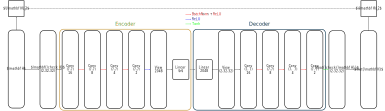
\includegraphics[width=.9\textwidth]{csinet-pro.pdf}
  % \medskip
  \caption{SphNet -- CsiNet-Pro architecture with Spherical Normalization.}
  \label{fig:sphnet-arch}
\end{figure}

\subsection{Results}
Training on spherically normalized data and optimizing with respect to NMSE can yield better accuracy. Fig.~\ref{fig:nmse_slot1} demonstrates this improvement for CsiNet and CsiNet-Pro on the COST2100 dataset. CsiNet and CsiNet-Pro are trained with minmax normalization while CsiNet-Sph and SphNet are trained with spherical normalization. % For both networks, the number of 

\begin{figure}[!hbtp] \centering 
	\begin{subfigure}[t]{.45\textwidth}
		\centering
		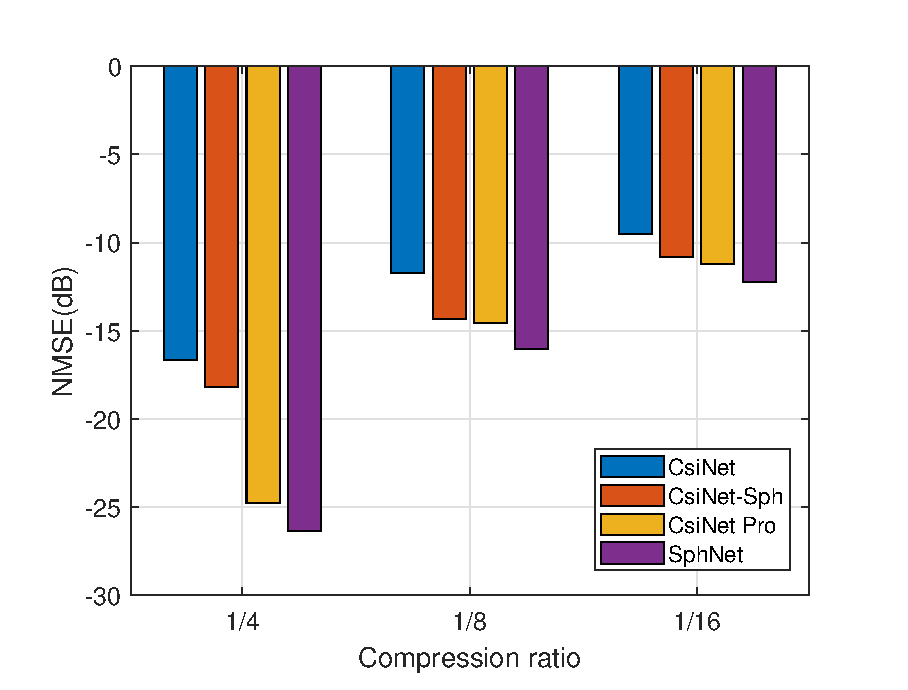
\includegraphics[width=\linewidth]{nmse_slot1_indoor.eps}
		\caption{Indoor}
		\label{fig:slot1_indoor} 
	\end{subfigure}
	\begin{subfigure}[t]{.45\textwidth}
		\centering
		\includegraphics[width=\linewidth]{nmse_slot1_outdoor.eps}
		\caption{Outdoor}
		\label{fig:slot1_outdoor} 
	\end{subfigure}
	\caption{Reconstruction error for CsiNet \cite{ref:csinet} and CsiNet Pro with and without spherical normalization. SphNet combines CsiNet Pro with spherical normalization \cite{ref:liu2020sphnet}.}
	\label{fig:nmse_slot1} 
\end{figure}


\chapter{Temporal Coherence}
\label{chap:markovnet}

% 03_markovnet.tex
% \section{Temporal Coherence in Time-varying Channels}
In this chapter, we consider methods for exploiting temporal correlation between CSI of subsequent timeslots. The \emph{coherence time} of a channel is the amount of time that a channel estimate can be used before that estimate's SNR falls beneath a given threshold \cite{ref:Chopra2016ChannelAging}. Within this window of time ($\Delta t = t_i - t_{i-1}$), the correlation between CSI matrices $\mathbf H_{i}$ and $\mathbf H_{i-1}$ is high (see Figure~\ref{fig:csi_img_gt} for an illustrative example). 
% Works exploiting temporal coherence use CSI matrices from previous timeslots to supplement subsequent estimates \cite{ref:Wang2019CsiNetLSTM}.

\begin{figure}[htb] \centering 
  % \includegraphics[width=0.9\linewidth]{batch0_csi_gt.png}
{
  \fontsize{10pt}{12pt}
  \def\svgwidth{1.0\columnwidth}
  \input{../images/batch0_csi_gt.pdf_tex}
}
  \caption{Ground truth CSI ($\mathbf H$) for five timeslots ($t_1$ through $t_5$) on one sample from the validation set of the outdoor dataset.} 
  \label{fig:csi_img_gt} 
\end{figure}

% Other works in channel state estimation exploit temporal coherence.

Assuming the channel exhibits temporal coherence within a certain window of time,
a reasonably accurate CSI estimate at time $t_{i-1}$ can be used to estimate the CSI at time $t_i$.
Generically, we can write this estimator as
\begin{align}
\grave{\mathbf H}_i &= h(\hat{\mathbf H}_{i-1}) \label{eq:gen_estim}
\end{align}
where $\mathbf{H}_i$ is the CSI matrix at time $t_i$ and $\hat{\mathbf H}_i$ is its estimator. 
The estimation error under $\grave{\mathbf H}_i$ is
\begin{align}
\mathbf E_{i} &= \mathbf H_{i} - \grave{\mathbf H}_{i}. \label{eq:diff_err}
\end{align}

\section{Recurrent Neural Networks}

Prior work in temporal correlation for CSI estimation utilized state-space methods such as the Kalman filter \cite{ref:Huber2006improved,ref:Ali2020BayesKalmanFilter,ref:Kim2021KalmanVsML}. Since it relies on explicit state space and noise models, the Kalman filter's predictive power in CSI estimation is limited. Furthermore, such work generally does not propose a method for feedback compression, making comparison with the following ML methods difficult.

Recent works have leveraged recurrent neural networks (RNNs) to exploit temporal correlation for CSI estimation \cite{ref:Lu2019RecCsiNet, ref:Liao2019BiLSTM, ref:Li2020SpatTempLSTM,
 ref:Jang2019Delay,ref:Wang2019CsiNetLSTM}. RNNs include recurrent layers, such as the long short-term memory (LSTM) cell or the gated recurrent unit (GRU), which are capable of learning long-term dependencies of a given process through backpropagation \cite{ref:Hermans2013Training} and can be used to predict future states of the process \cite{ref:Pascanu2014HowTo}.

\begin{figure}[htb]
	\centering
	\includegraphics[width=.9\textwidth]{lstm-example-unroll.pdf}
	\medskip
	\caption{An example of LSTMs used for CSI estimation. (a) ``Stacked'' LSTM network of depth 3 shown with recurrent connections. (b) Same LSTM network ``unrolled" into $T$ timeslots }
	\label{fig:lstm_example}
\end{figure}

RNNs have been used extensively in natural language processing (NLP) for machine translation \cite{ref:Sutskever2014seq2seq} and sentiment extraction \cite{ref:Irsoy2014opinion}. For such works in NLP, authors have empirically found ``stacked'' or ``deep'' RNNs to be effective (e.g., Fig.~\ref{fig:lstm_example}), hypothesizing that having multiple recurrent layers allows the network to extract different semantic timescales \cite{ref:Irsoy2014opinion, ref:Bengio2009Learning}. Works in CSI estimation have taken cues from this work in NLP, proposing CSI estimation networks with stacked LSTMs after a sequence of autoencoders \cite{ref:Wang2019CsiNetLSTM}. While such work has demonstrated the utility of RNNs, the computational cost of LSTMs can be prohibitively high. For example, the RNN portion of the network proposed in \cite{ref:Wang2019CsiNetLSTM} accounts for $10^8$ additional parameters. Since channel estimation should not place an undue computational burden on the communications system, LSTMs can be problematic.

\section{Differential Encoding}

Rather than use RNNs to extract temporal dependencies in CSI data, we proposed a lightweight network based on the principle of differential encoding. We trained a network to estimate the error (\ref{eq:diff_err}) under a linear estimator, 
\begin{align*}
	\grave{\mathbf H}_i &=  \hat{\mathbf H}_{i-1} \mathbf W
\end{align*}
where $\mathbf W \in \mathbb C^{R_b \times R_b}$ is the minimum mean squared error (MMSE) estimator,
\begin{align*}
	\mathbf H_i &= \mathbf H_{i-1}\mathbf W + \mathbf E_i \\
	\mathbf H_{i-1}^H\mathbf H_i &= \mathbf H_{i-1}^H\mathbf H_{i-1} \mathbf W + \cancelto{\mathbf 0}{\mathbf H_{i-1}^H\mathbf E_i}
\end{align*}
where the cancellation of the product $\mathbf H_{i-1}^H\mathbf E_i$ is due to the principle of orthogonality (i.e., the error terms are orthogonal to the observed data). Denoting the cross correlation matrix as $\mathbf R_{i} = \mathbb{E}\left[\mathbf H_{t-i}^H\mathbf H_{t}\right]$, we solve for the MMSE estimator,
\begin{align*}
	\mathbf W &= \mathbf R_0^{-1} \mathbf R_1.
\end{align*}
In practice, the population correlation matrices are estimated
via finite samples of size $N$,
\begin{align*}
	\mathbf{\hat R}_k &= \frac 1N \sum_{j}^N \mathbf H_{i-k}^H(j)\mathbf H_{i}(j),
\end{align*}
where $\mathbf H_i(j)$ is the $j$-th sample in the training set.
The MMSE estimator based on the sample correlation matrices is written as
\begin{align*}
	\hat{\mathbf W} &= \hat{\mathbf R}_0^{-1} \hat{\mathbf R}_1.
\end{align*}
We can further simplify this estimator to a scalar, $\gamma \in \mathbb R$, as
% \begin{align*}
%   \hat \gamma &= \frac{\sum_{i=1}^N\text{Trace}(\left[\mathbf H_{t-1}^H(i)\mathbf H_{t}(i)\right])}{\sum_{i=1}^N\Arrowvert\mathbf H_t^H(i) \mathbf H_t(i)\Arrowvert^2},
% \end{align*}
\begin{align*}
	\hat \gamma &= \frac{\text{Trace}(\hat{\mathbf R}_1(k,l))}{\sum_k^{R_d}\sum_l^{N_b}\hat{\mathbf R}_0(k,l)},
\end{align*}
where $k$ ($l$) are the row (column) indices of the correlation matrices. The estimator in this case is 
\begin{align}
	\grave{\mathbf H}_i &= \hat\gamma \hat{\mathbf H}_{i-1} \label{eq:gamma-estim}.
\end{align}
Under the estimator $\gamma$, we proposed to encode the error, $\mathbf E_t$, using a convolutional autoencoder, $f(\mathbf E_t)$,
\begin{align*}
	\hat{\mathbf E}_i &= g(f(\mathbf E_i, \vec\theta_e), \vec\theta_d),
\end{align*}
where $\mathbf E_i = \mathbf H_i - \gamma\hat{\mathbf H}_{i-1}$. The base station has access to the estimators $\gamma$ and $\hat{\mathbf H}_{i-1}$, and the resulting CSI estimate at $t_i$ is
\begin{align}
	\hat{\mathbf H}_i &= \hat\gamma \hat{\mathbf H}_{i-1} + \hat{\mathbf{E}}_i \label{eq:diff-estim}
\end{align}

\subsection{MarkovNet}

In \cite{ref:Liu2020MarkovNet}, we proposed MarkovNet, a deep differential autoencoder. Each timeslot of MarkovNet uses an instance of CsiNet-Pro with unique parameters. The network at the first timeslot ($t_1$) is trained directly on the CSI ($\mathbf H_1$). For all subsequent timeslots, $t_i$ for $i \geq 2$, we use the MMSE estimator (\ref{eq:gamma-estim}) to produce an error term $\mathbf E_t$, and the autoencoder in each timeslot is trained to produce an error estimate, $\hat{\mathbf E}_t$. The estimated error is added back per (\ref{eq:diff-estim}) to produce a refined estimate.

\begin{figure}[!hbtp]
    \centering
    {
      \fontsize{6pt}{8pt}
      \def\svgwidth{0.8\columnwidth}
      \input{../images/markovnet_schematic.pdf_tex}
    }
    \caption{Abstract architecture for MarkovNet. Networks at $t_i$ for $i \geq 2$ are trained to predict the estimation error, $\mathbf E_i$.}
    \label{fig:markovnet_schema}
\end{figure}

The resulting network requires no recurrent layers, resulting in a substantial reduction in computational complexity. Table~\ref{tab:comp-complex} shows the number of parameters and FLOPs per timeslot for CsiNet-LSTM, MarkovNet, and CsiNet. The parameter count of MarkovNet is on par with CsiNet, and CsiNet-LSTM requires orders of magnitude more parameters. While the number of FLOPs for MarkovNet is nearly 10 times smaller than CsiNet-LSTM, MarkovNet requires 5 to 10 times more FLOPs than CsiNet due to the increased kernel size of CsiNet-Pro.

\begin{table}[htb]
  \renewcommand{\arraystretch}{1}
  \begin{center}
  % \caption{Table II: Model size \& computational complexity comparison. M: million, K: thousand.}
  \caption{Model size/computational complexity of tested temporal networks (CsiNet-LSTM, MarkovNet) and comparable non-temporal network (CsiNet). M: million.}
  \label{tab:comp-complex} 
  % \resizebox{\linewidth}{15mm}
  \footnotesize{
	  \begin{tabular}{|l|c|c|c|c|c|c|}
	  \hline
	                              & \multicolumn{3}{c|}{\textbf{Parameters}} & \multicolumn{3}{c|}{\textbf{FLOPs}} \\ \hline
	                              & \textbf{CsiNet-LSTM} & \textbf{MarkovNet} & \textbf{CsiNet} & \textbf{CsiNet-LSTM} & \textbf{MarkovNet} & \textbf{CsiNet} \\ \hline
	  \textbf{CR=$1/4$}  		  & 132.7 M              & 2.1 M              & 2.1 M  			& 412.9 M              & 44.5 M             & 7.8 M           \\ \hline
	  \textbf{CR=$1/8$}  		  & 123.2 M              & 1.1 M              & 1.1 M  			& 410.8 M              & 42.	4 M             & 5.7 M           \\ \hline
	  \textbf{CR=$1/16$} 		  & 118.5 M              & 0.5 M              & 0.5 M 			& 409.8 M              & 41.3 M             & 4.7 M           \\ \hline
	  \textbf{CR=$1/32$} 		  & 116.1 M              & 0.3 M              & 0.3 M           & 409.2 M              & 40.8 M             & 4.1 M           \\ \hline
	  \textbf{CR=$1/64$} 		  & 115.0 M              & 0.1 M              & 0.1 M 			& 409.0 M              & 40.5 M             & 3.9 M           \\ \hline
	  \end{tabular}
  }
  \end{center}
\end{table} 

\subsection{Results}

We compare MarkovNet with CsiNet-LSTM \cite{ref:Wang2019CsiNetLSTM} on the indoor and outdoor COST2100 datasets (for details, see Section~\ref{sect:channel_model}). For MarkovNet, we train the network at the first timeslot for 1000 epochs. In each subsequent timeslot, we initialize the network using the weights from the previous timeslot and train for 200 epochs. We use a batch size of 200. We perform a training/testing split of 75k/25k samples, and we estimate $\gamma$ using the training set. To compare the estimation accuracy of each network, we report the NMSE.
%estimate of the previous timeslot with the scalar MMSE estimator, $\gamma$, to produce the error term $\mathbf E_t = \mathbf H_t - \gamma\hat{\mathbf H}_{t-1}$.

Figure~\ref{fig:diffnet_result} shows the NMSE of MarkovNet and CsiNet-LSTM for four different compression ratios. For the indoor network, all instances of MarkovNet achieve lower NMSE than all instances of CsiNet-LSTM. In the outdoor scenario, each CR for MarkovNet demonstrates lower NMSE than the corresponding CR for CsiNet-LSTM. Between both channel scenarios, MarkovNet shows gradual improvement for subsequent timeslots if the CR is high enough while CsiNet-LSTM only improves gradually in the outdoor environment for CR$=\frac 14$.
\begin{figure}[!hbtp] \centering 
	\begin{subfigure}[t]{.45\textwidth}
		\centering
		\includegraphics[width=\linewidth]{MarkovNet_truncated_Indoor_10slots.pdf}
		\caption{Indoor}
		\label{fig:diffnet_indoor} 
	\end{subfigure}
	\begin{subfigure}[t]{.45\textwidth}
		\centering
		\includegraphics[width=\linewidth]{MarkovNet_truncated_Outdoor_10slots.pdf}
		\caption{Outdoor}
		\label{fig:diffnet_outdoor} 
	\end{subfigure}
	\caption{$\text{NMSE}$ comparison of MarkovNet and CsiNet-LSTM 
	at various compression ratios (CR).} 
	\label{fig:diffnet_result} \vspace*{-2mm}
\end{figure}  
Figure~\ref{fig:csi_image} shows a random sample from the test set, $\mathbf H$, and the estimates produced by CsiNet-LSTM and MarkovNet for a CR of $\frac 14$. This sample contains three ``peak'' magnitude regions. While both networks manage to capture the two larger samples, MarkovNet is able to recover the small peak magnitude region ({\color{darkgreen}green arrow}) which CsiNet-LSTM fails to produce ({\color{red}red arrow}).

\begin{figure}[htb] \centering 
	\includegraphics[width=0.9\linewidth]{batch0_csi_compare_cr512_annot.pdf}
	\caption{CSI ($\mathbf H$), MarkovNet estimates ($\hat{\mathbf H}_{\text{Markov}}$), and CsiNet-LSTM estimates ($\hat{\mathbf H}_{\text{LSTM}}$) across five timeslots ($T_1$ through $T_5$) on one outdoor channel sample from the test set,
using $\text{CR}=\frac 14$.} 
	\label{fig:csi_image} 
\end{figure}

\chapter{Feedback Quantization}
\label{chap:csinet_quant}
% 04_csinet_quant.tex



While previous works investigated neural architectures for learned encoding-decoding of CSI data, such architectures rely on continuous valued latent representations (codewords). The use of such continuous codewords presents at least two issues:
\begin{enumerate}
	\item \textbf{Quantization}: Modulation protocols require quantized data to accommodate bit string representations and IQ constellations. To make neural autoencoders compatible with common modulation schemes, trainable CSI compression techniques should incorporate quantized codewords in the learning process.
	\item \textbf{Metrics for Compressibility}: Works in learnable CSI compression typically present a given network's reconstruction error a range of compression ratios (e.g., \cite{ref:csinet,ref:dualnet}) but do not discuss the network's compatibility with coding schemes. Coding techniques such as arithmetic coding \cite{ref:Witten1987Arithmetic}) require probability estimates of the encoded symbols in order to operate \cite{ref:Howard1994Arithmetic}. Based on Shannon's coding theorem \cite{ref:Shannon1948Mathematical}, the entropy of the encoded alphabet establishes is the minimum transmission rate needed to encode a given symbol. To describe their compatibility with optimal coding schemes, neural CSI compression techniques should be presented with the entropy of their encoded alphabets in order to assess the realized encoding distributions.
	% theory give metrics such entropy and mutual information which quantify the information in a given distribution.
\end{enumerate}

\subsection{Related Work}

Prior work has investigated feedback quantization in deep learning-based CSI compression. In \cite{ref:Yang2019DeepCMC}, the authors propose DeepCMC, an autoencoder structure where the continuous compressed elements are discretized via uniform quantization then encoded using context adaptive binary arithmetic coding (CABAC) \cite{ref:Marpe2003CABAC}. Since uniform quantization is non-differentiable, the authors do not perform true quantization during training and instead apply uniformly distributed noise to approximate quantization noise \cite{ref:Yang2019DeepCMC}. In \cite{ref:Mashhadi2020AnalogDeepCMC}, the authors propose AnalogDeepCMC, which encodes latent elements as power-normalized complex elements and decodes using maximal ratio combining. The authors also report the achieved rate of AnalogDeepCMC for different CSI overhead ratios.

To achieve discrete codewords with valid probability distributions, we consider works in neural discrete representations. In \cite{ref:Oord2017Neural}, the authors propose \emph{vector quantization (VQ)}, which partitions a $r$-dimensional latent space into $d$-dimensional vectors and quantizes the latent space based on a nearest neighbor assignment. In \cite{ref:Agustsson2017SoftToHard}, the authors proposed soft-to-hard VQ (SHVQ), a softmax relaxation of VQ which enables a latent entropy term which can be used to regularize the loss function.  Unlike the prior work, SHVQ allows for end-to-end training with feedback quantization.

\begin{figure}[!hbtp]
\centering
\def\svgwidth{0.8\columnwidth}
\input{../images/csinet_quant.pdf_tex}
\caption{Abstract architecture for CsiNet-Quant. SoftQuantize layer ($Q(\tilde{\mathbf Z})$) is a continuous, softmax-based relaxation of a $d$-dimensional quantization of the latent layer $\mathbf Z$.}
\label{fig:csinet_quant}
\end{figure}

\subsection{A Vector Quantized Autoencoder for Trainable Codewords}
% \subsubsection{CsiNet-Quant: A Vector Quantized Autoencoder for Trainable Codewords}

To incorporate discrete latent codewords in the learning process, we propose to use soft-to-hard vector quantization framework proposed in \cite{ref:Agustsson2017SoftToHard}. We choose a vector dimension, $m$, by which to partition the latent space $\mathbf Z = f(\mathbf H, \theta_e)$, and we denote the vectorized version of $\mathbf Z \in \mathbb R^{r}$ as $\tilde{\mathbf Z} \in \mathbb R^{r/m \times m}$. We define the $m$-dimensional codebook of size $L$ as $\mathbf C \in \mathbb R^{m\times L}$. The soft assignments of the $j$-th latent vector $\tilde{\mathbf z}_j$ can be written as
\begin{align}
\phi(\tilde{\mathbf z}_j) &= \left[\frac{\text{exp}(-\sigma \Arrowvert \tilde{\mathbf z}_j - \mathbf c_\ell\Arrowvert^2)}{\sum_{i=1}^L\text{exp}(-\sigma \Arrowvert \tilde{\mathbf z}_j - \mathbf c_i\Arrowvert^2)}\right]_{\ell\in [L]} \in \mathbb R^L \label{eq:soft_assign}
\end{align}
(\ref{eq:soft_assign}) is typically referred to as the \emph{softmax} function, which is commonly used as a differentiable alternative to the maximum function in deep learning. The hyperparameter $\sigma$ controls the temperature of the softmax scores, with a lower $\sigma$ yielding a more uniform distribution and a higher $\sigma$ yielding a ``peakier'' distribution (i.e., $\sigma \to \infty \Rightarrow \phi(\tilde z_j) \to \text{max}(\tilde z_j)$). Using the soft assignments, the latent vectors are quantized based on the codewords $\mathbf C \in \mathbb R^{m \times L}$,
\begin{align}
Q(\tilde{\mathbf z}_j,\mathbf C) &= \phi(\tilde{\mathbf z}_j) \mathbf C^T. \label{eq:soft_quant}
\end{align}
The quantized version of the latent variable is taken by reshaping $\mathbf Q(\tilde{\mathbf Z},\mathbf C) \in \mathbb R^{r/m \times m}$ into $\hat{\mathbf Z} \in \mathbb R^d$, and the decoder produces the CSI estimates as $\hat{\mathbf H} = h(\hat{\mathbf Z}, \mathbf C)$. An abstract illustration of an autoencoder using soft quantization can be seen in Figure~\ref{fig:csinet_quant}.

\subsubsection{Entropy-regularization}
To optimize the network with soft quantization, we adapt the loss function to resemble the canonical rate-distortion function by adding an entropy penalization term,
\begin{align}
\underset{\theta_e, \theta_d, \mathbf C}{\text{argmin}}\; \frac 1N \underbrace{\sum_{i=1}^N\Arrowvert \mathbf H_i - g(Q(f(\mathbf H_i, \theta_e), \mathbf C), \theta_d) \Arrowvert^2}_{\text{distortion loss}} + \underbrace{\lambda \left(\Arrowvert\theta_e\Arrowvert^2+\Arrowvert\theta_d\Arrowvert^2+\Arrowvert \mathbf C \Arrowvert^2\right)}_{\ell^2\text{ penalty}} + \underbrace{m\beta H(\phi)}_{\text{rate loss}}. \label{eq:loss_entropy}
\end{align}
Where $H(\phi)=H(p,q)$ is the crossentropy based on the hard and soft probability estimates $p$ and $q$, respectively. Before defining the estimates $p$ and $q$, we briefly discuss the population probabilities of the latent codewords. Denote the symbol encoder/decoder pair as $E:\mathbb R^m \to [L]^m$/$D:[L]^m \to \mathbb R^m$. Denote the distribution of latent variables as $\mathsf Z$ such that $\mathbf z \sim \mathsf Z$ with the encoder $E(\mathsf Z)=\mathbf e$ . The entropy of $\mathsf Z$ is given as 
\begin{align*}
H(E(\mathsf Z)) &= -\sum_{\mathbf e\in[L]^m}P(E(\mathsf Z) = \mathbf e)\log_2(P(E(\mathsf Z)=\mathbf e)).
\end{align*}
% The true probabilities over the latent vectors as $p_j$ with entropy $H(p) = -\sum_{j}^m p_j\log_2 p_j$.
In practice, the true population probabilities $P(E(\mathsf Z))$ are inaccessible, and we must estimate the probability masses via finite sampling over the encoder's outputs, $e(\mathbf z)$. The hard probability estimate $p_j$ of the $j$-th codeword is
\begin{align*}
p_j &= \frac{|\{e_l(\mathbf z_i)|l\in[m], i \in [N], e_l(\mathbf z_i)=j\}|}{mN}.
\end{align*}
The soft assignments of $\phi$ admit valid probability masses, $q_j = \phi(\tilde{\mathbf z})$, over the codewords. Using histogram estimates $p_j$ and the soft assignments $q_j$, the crossentropy term is written
\begin{align*}
H(\phi) := H(p,q) &= -\sum_{j=1}^L p_j\log q_j = H(p) + D_{\text{KL}}(p\Arrowvert q)
\end{align*}
where $D_{\text{KL}}(p\Arrowvert q)=-\sum_{j=1}^L p_j \log\left(\frac{p_j}{q_j}\right)$ is the Kullback Liebler (KL) divergence. Due to the nonnegativity of $D_{\text{KL}}$, $H(\phi)$ is an upper bound on $H(p)$, and so (\ref{eq:loss_entropy}) is a valid optimization target.

The mean squared error of the soft (hard) network is given as $e_S=\Arrowvert \tilde F(\mathbf H) - \mathbf H\Arrowvert^2$ ($e_H=\Arrowvert \hat F(\mathbf H) - \mathbf H\Arrowvert^2$), and the performance gap is given as $\text{gap}(t)=e_H - e_S$.

\subsection{Results}

We use SHVQ \cite{ref:Agustsson2017SoftToHard} to perform quantization on different CSI estimation networks. We used the COST2100 data introduced in Section~\ref{sect:channel_model}. We train the network in three stages:
\begin{enumerate}
	\item \textbf{Autoencoder pretraining}: Training the autoencoder ($\hat{\mathbf{H}}=g(f(\mathbf H, \vec\theta_e), \vec\theta_d)$) without latent quantization (1000 epochs). The autoencoder is trained with the MSE objective function.
	\item \textbf{Center pretraining}: Training soft quantization layer to initialize centers, $\mathbf C$ (1000 epochs). Using $\vec \theta_e$ from stage 1, the soft quantizer is trained on $\mathbf Z=f(\mathbf H, \vec \theta_e)$ to minimize the cluster energy, $\underset{\mathbf C}{\text{argmin}}\sum_{i=1}^N \Arrowvert \tilde{\mathbf Z} - Q(\tilde{\mathbf Z})\Arrowvert^2$.
	\item \textbf{SHVQ finetuning}: Using the results of stage 1 ($\vec\theta_e, \vec\theta_d$) and stage 2 ($\mathbf C$), we finetune the autoencoder and the soft quantization layer (50 epochs). The soft-quantized autoencoder is trained with the entropy-regularized MSE (Equation (\ref{eq:loss_entropy})).
\end{enumerate}

We use a batch size of 200. We perform a training/testing split of 75k/25k sample. For stage 3, we sweep the parameter $\beta$ to realize different latent entropy values $H(\phi)$. To visualize the rate-distortion of the proposed network, we show the network's NMSE versus the bits per pixel (bpps), 
\begin{align*}
	\text{bpps}	 &= \frac{rm}{2 n_{b}R_{d}}H(\phi) = CR\times mH(\phi). % bpps = test_entropy * (model.latent_dim / model.quant.m) / (2*model.decoder.img_total) # bits per pixel
\end{align*}
We also perform experiments with arithmetic encoding on the hard quantized centers, and we report the resulting bits per pixel as
\begin{align*}
	\text{bpps}	 &= \frac{\frac 1N \sum_{i}^N b_{\text{AE}}}{2 n_{b}R_{d}}. % bpps = test_entropy * (model.latent_dim / model.quant.m) / (2*model.decoder.img_total) # bits per pixel
\end{align*}
where $b_{\text{AE}}$ is the average bits per feedback message under arithmetic encoding.

We demonstrate the performance of CsiNet, SphNet, and DualNet-MAG under latent quantization. Table~\ref{tab:quant-params} summarizes the parameters used in these tests.

\begin{table}[]
\centering
\caption{Parameters/hyperparameters used for CsiNet-Quant.}
\label{tab:quant-params}
\begin{tabular}{c|c|l}
\toprule
\textbf{Symbol}   & \textbf{Values}  & \textbf{Description} \\ \midrule
$L$ 		  	  & $1024$	 		 & Number of centers/codewords for VQ.  \\ \hline
$d$               & $4$				 & Dimensionality of vectors in VQ.  \\ \hline
$r$               & $4$				 & Number of elements at the encoder's output (i.e., dimension of latent layer).  \\ \hline
\end{tabular}
\end{table}

\subsubsection{Rate-Distortion}

Figures~\ref{fig:rate-distortion-minmax} and~\ref{fig:rate-distortion-sph} show the performance of CsiNet-Quant under minmax and spherical normalization, respectively. 

\begin{figure}[htb] \centering 
  \includegraphics[width=0.8\linewidth]{rate-distortion-all-cr-H4.pdf}
  \caption{Rate distortion of CsiNet-Quant under minmax normalization using: $L=1024$ centers, $d=4$. Hard, soft, and no quantization performance shown for each CR.} 
  \label{fig:rate-distortion-minmax} 
\end{figure}

\begin{figure}[htb] \centering 
  \includegraphics[width=0.8\linewidth]{rate-distortion-all-cr-sphH4.pdf}
  \caption{Rate distortion of CsiNet-Quant under spherical normalization using: $L=1024$ centers, $d=4$. Hard, soft, and no quantization performance shown for each CR.} 
  \label{fig:rate-distortion-sph} 
\end{figure}

\begin{figure}[htb] \centering 
  \includegraphics[width=0.8\linewidth]{rate-distortion-all-norm.pdf}
  \caption{Rate distortion under hard quantization for both minmax (dotted line) and spherical (solid line) normalization using.} 
  \label{fig:rate-distortion-norms} 
\end{figure}

% Open Questions:
% Metrics for Compressibility:
% - Rate calculation: Can depend on
% 	- Precoding technique (conjugate beamforming, zero-forcing)
% 	- SNR in Uplink/Downlink
% - Entropy:
%	- Latent entropy estimation enables rate-loss
% 	- Raw entropy estimation techniques?
%		- Discrete: Questions of quantization resolution
%		- Continuous: Questions of hyperparameters for density-estimatiors (i.e., KNN)
% - Realized Bitrate under Entropy Encoding
% 	- Given rate-regularized training, what is the average Tx bit rate under an entropy encoding scheme?
% 		- Start with Arithmetic Codin
%		- Move onto Context-adaptive binary arithmetic coding

\chapter{Conclusion}
% 05_conclusion.tex

\blindtext


\newpage
\small
\bibliographystyle{ieeetr}
\bibliography{../cited_works}

\end{document}